% =============================================================================
% PhishGuard — BSc Thesis Defense
% Author: Ishaq Muhammad (PXPRGK) · ELTE Faculty of Informatics · June 2026
% =============================================================================
\documentclass[aspectratio=169,10pt]{beamer}

% ── Theme ──────────────────────────────────────────────────────────
\usetheme{metropolis}
\setbeamercolor{background canvas}{bg=white}

% Override metropolis colors — clean, professional palette
\definecolor{primary}{HTML}{1B3A5C}      % deep navy
\definecolor{accent}{HTML}{2E86AB}       % steel blue
\definecolor{danger}{HTML}{C0392B}       % muted red
\definecolor{success}{HTML}{1E8449}      % muted green
\definecolor{warning}{HTML}{D4A017}      % muted gold
\definecolor{dark}{HTML}{2C3E50}         % dark text
\definecolor{graybg}{HTML}{F5F6FA}       % light gray card bg
\definecolor{border}{HTML}{D5D8DC}       % subtle border

\setbeamercolor{frametitle}{bg=white,fg=primary}
\setbeamercolor{title separator}{fg=accent}
\setbeamercolor{progress bar}{fg=accent}
\setbeamercolor{block title}{bg=primary,fg=white}
\setbeamercolor{block body}{bg=graybg,fg=dark}
\setbeamercolor{block title example}{bg=success,fg=white}
\setbeamercolor{block body example}{bg=graybg,fg=dark}
\setbeamercolor{block title alerted}{bg=danger,fg=white}
\setbeamercolor{block body alerted}{bg=graybg,fg=dark}
\setbeamercolor{normal text}{fg=dark}
\setbeamercolor{alerted text}{fg=danger}
\setbeamercolor{example text}{fg=success}

% ── Fonts ──────────────────────────────────────────────────────────
\usepackage{lmodern}
\usepackage{textcomp}
\usepackage[T1]{fontenc}
\usefonttheme{professionalfonts}
\setbeamerfont{frametitle}{size=\Large,series=\bfseries}
\setbeamerfont{block title}{size=\normalsize,series=\bfseries}

% ── Packages ───────────────────────────────────────────────────────
\usepackage{graphicx}
\usepackage{booktabs}
\usepackage{colortbl}
\usepackage{xcolor}
\usepackage{tikz}
\usetikzlibrary{positioning}

% ── Footer — clean, minimal ────────────────────────────────────────
\setbeamertemplate{frame footer}{\hspace{1em}\color{gray!60}\footnotesize\insertshortauthor\ \ $\vert$\ \insertshorttitle\ \ $\vert$\ \insertframenumber}

% ── Spacing ────────────────────────────────────────────────────────
\setlength{\parskip}{0.6em}

% ── Title ──────────────────────────────────────────────────────────
\title{PhishGuard}
\subtitle{Hybrid ML + OSINT Architecture for\\Proactive Phishing Detection}
\author{Ishaq Muhammad}
\institute{Eötvös Loránd University · Faculty of Informatics\\BSc Thesis Defense · June 2026}
\date{}

% =============================================================================
\begin{document}

% ═══════════════════════════════════════════════════════════════════
\maketitle

% ═══════════════════════════════════════════════════════════════════
\begin{frame}{The Problem}
  \vspace{0.3cm}
  \begin{columns}[T]
    \column{0.48\textwidth}
      \begin{block}{Phishing is accelerating}
        \begin{itemize}
          \setlength{\itemsep}{0.4em}
          \item \textbf{\$10.3 billion} annual losses (FBI)
          \item \textbf{1.2M+} unique phishing sites in 2023
          \item \textbf{80\%+} of phishing sites now use HTTPS
        \end{itemize}
      \end{block}
    \column{0.48\textwidth}
      \begin{alertblock}{Blacklists are too slow}
        \begin{itemize}
          \setlength{\itemsep}{0.4em}
          \item Must be \textbf{reported \& verified} first
          \item \textbf{50\%} of phishing domains last \textbf{$<$ 12 hours}
          \item Zero-day attacks hit \emph{before} blacklists update
        \end{itemize}
      \end{alertblock}
  \end{columns}
  \vspace{0.3cm}
  \begin{block}{Existing ML models are \textbf{context-blind}}
    A URL like \texttt{secure-login-chase-update.com} looks structurally normal.
    Only live intelligence reveals: \textbf{registered 2 days ago}, \textbf{no email configured}, \textbf{privacy-protected}.
  \end{block}
\end{frame}

% ═══════════════════════════════════════════════════════════════════
\begin{frame}{Our Approach}
  \vspace{0.3cm}
  \begin{center}
    \Large\textbf{Combine three intelligence layers into one explainable verdict.}
  \end{center}
  \vspace{0.4cm}
  \begin{columns}[T]
    \column{0.31\textwidth}
      
\begin{tikzpicture}
        \node[draw=primary,fill=primary!5,rounded corners=6pt,inner sep=14pt,text width=0.95\columnwidth,align=center] {
          {\large\color{primary}\textbf{Machine Learning}}\\[0.4em]
          XGBoost classifier\\21 features\\96.5\% accuracy\\0.1ms inference
        };
      \end{tikzpicture}
    \column{0.31\textwidth}
      
\begin{tikzpicture}
        \node[draw=accent,fill=accent!5,rounded corners=6pt,inner sep=14pt,text width=0.95\columnwidth,align=center] {
          {\large\color{accent}\textbf{OSINT}}\\[0.4em]
          Live WHOIS \& DNS\\VirusTotal \& AbuseIPDB\\15s parallel timeout\\Graceful fallback
        };
      \end{tikzpicture}
    \column{0.31\textwidth}
      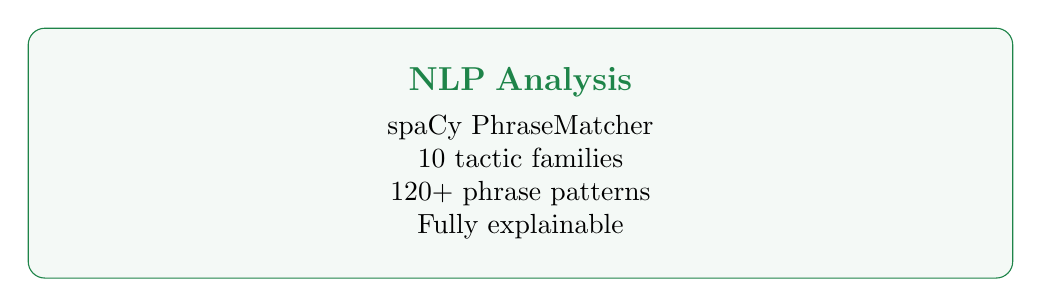
\begin{tikzpicture}
        \node[draw=success,fill=success!5,rounded corners=6pt,inner sep=14pt,text width=0.95\columnwidth,align=center] {
          {\large\color{success}\textbf{NLP Analysis}}\\[0.4em]
          spaCy PhraseMatcher\\10 tactic families\\120+ phrase patterns\\Fully explainable
        };
      \end{tikzpicture}
  \end{columns}
  \vspace{0.4cm}
  \begin{center}
    \large $\rightarrow$ \textbf{Verdict} (Safe · Suspicious · Dangerous · Critical) with confidence score \& human-readable reasons
  \end{center}
\end{frame}

% ═══════════════════════════════════════════════════════════════════
\begin{frame}{System Architecture}
  \vspace{-0.2cm}
  \begin{center}
    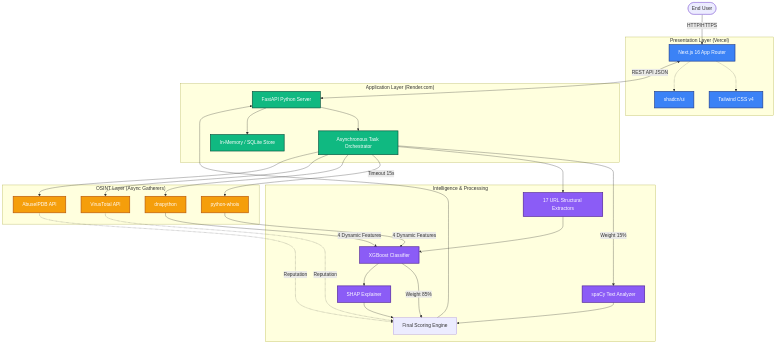
\includegraphics[height=0.78\textheight]{../latex_source/images/system-architecture.png}
  \end{center}
\end{frame}

% ═══════════════════════════════════════════════════════════════════
\begin{frame}[standout]
  \Large How do we train the model?
\end{frame}

% ═══════════════════════════════════════════════════════════════════
\begin{frame}{Data Pipeline}
  \vspace{0.3cm}
  \begin{center}
    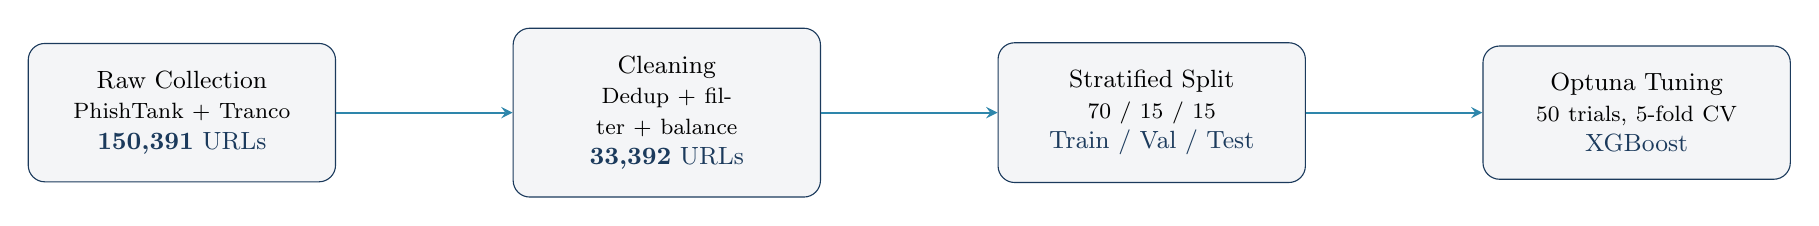
\begin{tikzpicture}[node distance=1.4cm,
      block/.style={draw=primary,fill=primary!5,rounded corners=6pt,inner sep=10pt,text width=3.2cm,align=center,font=\small},
      arrow/.style={->,>=stealth,thick,color=accent}]
      \node[block] (raw) {Raw Collection\\{\footnotesize PhishTank + Tranco}\\{\color{primary}\textbf{150,391} URLs}};
      \node[block] (clean) at ([xshift=4.2cm]raw.east) {Cleaning\\{\footnotesize Dedup + filter + balance}\\{\color{primary}\textbf{33,392} URLs}};
      \node[block] (split) at ([xshift=4.2cm]clean.east) {Stratified Split\\{\footnotesize 70 / 15 / 15}\\{\color{primary}Train / Val / Test}};
      \node[block] (train) at ([xshift=4.2cm]split.east) {Optuna Tuning\\{\footnotesize 50 trials, 5-fold CV}\\{\color{primary}XGBoost}};
      \draw[arrow] (raw.east) -- (clean.west);
      \draw[arrow] (clean.east) -- (split.west);
      \draw[arrow] (split.east) -- (train.west);
    \end{tikzpicture}
  \end{center}
  \vspace{0.3cm}
  \begin{block}{Final test set: \textbf{5,009} samples — perfectly balanced}
    \centering 2,505 legitimate \ $\vert$\  2,504 phishing
  \end{block}
\end{frame}

% ═══════════════════════════════════════════════════════════════════
\begin{frame}{21 Features — 17 Structural + 4 OSINT}
  \vspace{0.2cm}
  \begin{columns}[T]
    \column{0.5\textwidth}
      \begin{block}{17 URL Structural Features}
        \footnotesize
        \begin{tabular}{@{}ll@{}}
          \texttt{urlLength} & total URL length \\
          \texttt{domainLength} & domain name length \\
          \texttt{subdomainCount} & subdomain levels \\
          \texttt{pathDepth} & path segments \\
          \texttt{hasIpAddress} & IP as domain \\
          \texttt{hasAtSymbol} & @ in URL \\
          \texttt{hasDoubleSlash} & // in path \\
          \texttt{hasDashInDomain} & hyphen in domain \\
          \texttt{hasUnderscoreInDomain} & \\
          \texttt{isHttps} & HTTPS used? \\
          \texttt{hasPortNumber} & non-std port \\
          \texttt{hasSuspiciousTld} & .tk, .ml, .xyz \\
          \texttt{hasEncodedChars} & \% encoding \\
          \texttt{hasSuspiciousKeywords} & \\
          \texttt{digitRatio} & \\
          \texttt{specialCharCount} & \\
          \texttt{queryParamCount} & \\
        \end{tabular}
      \end{block}
    \column{0.5\textwidth}
      \begin{block}{4 OSINT Features}
        \footnotesize
        \begin{tabular}{@{}ll@{}}
          \texttt{hasValidMx} & mail configured? \\
          \texttt{usesCdn} & CDN masking? \\
          \texttt{dnsRecordCount} & DNS footprint \\
          \texttt{hasValidDns} & domain resolves? \\
        \end{tabular}
      \end{block}
      \vspace{0.4cm}
      \begin{exampleblock}{Key innovation}
        \small OSINT features live \textbf{inside} the ML vector —\\the model learns from \emph{real-time Internet state},\\not just static URL strings.
      \end{exampleblock}
  \end{columns}
\end{frame}

% ═══════════════════════════════════════════════════════════════════
\begin{frame}{Model Performance}
  \vspace{0.2cm}
  \begin{columns}[T]
    \column{0.42\textwidth}
      \begin{block}{Metrics — Test Set (5,009)}
        \large
        \begin{tabular}{@{}lr@{}}
          \toprule
          \textbf{Accuracy} & \textbf{96.45\%} \\
          \textbf{Precision} & \textbf{97.86\%} \\
          Recall & 94.97\% \\
          \textbf{F1-Score} & \textbf{96.39\%} \\
          \textbf{AUC-ROC} & \textbf{99.41\%} \\
          \bottomrule
        \end{tabular}
      \end{block}
      \vspace{0.3cm}
      \begin{block}{Optuna — Best Trial \#43}
        \footnotesize
        \begin{tabular}{@{}ll@{}}
          \texttt{max\_depth} & 7 \\
          \texttt{learning\_rate} & 0.177 \\
          \texttt{n\_estimators} & 700 \\
        \end{tabular}
      \end{block}
    \column{0.58\textwidth}
      \vspace{-0.2cm}
      \begin{center}
        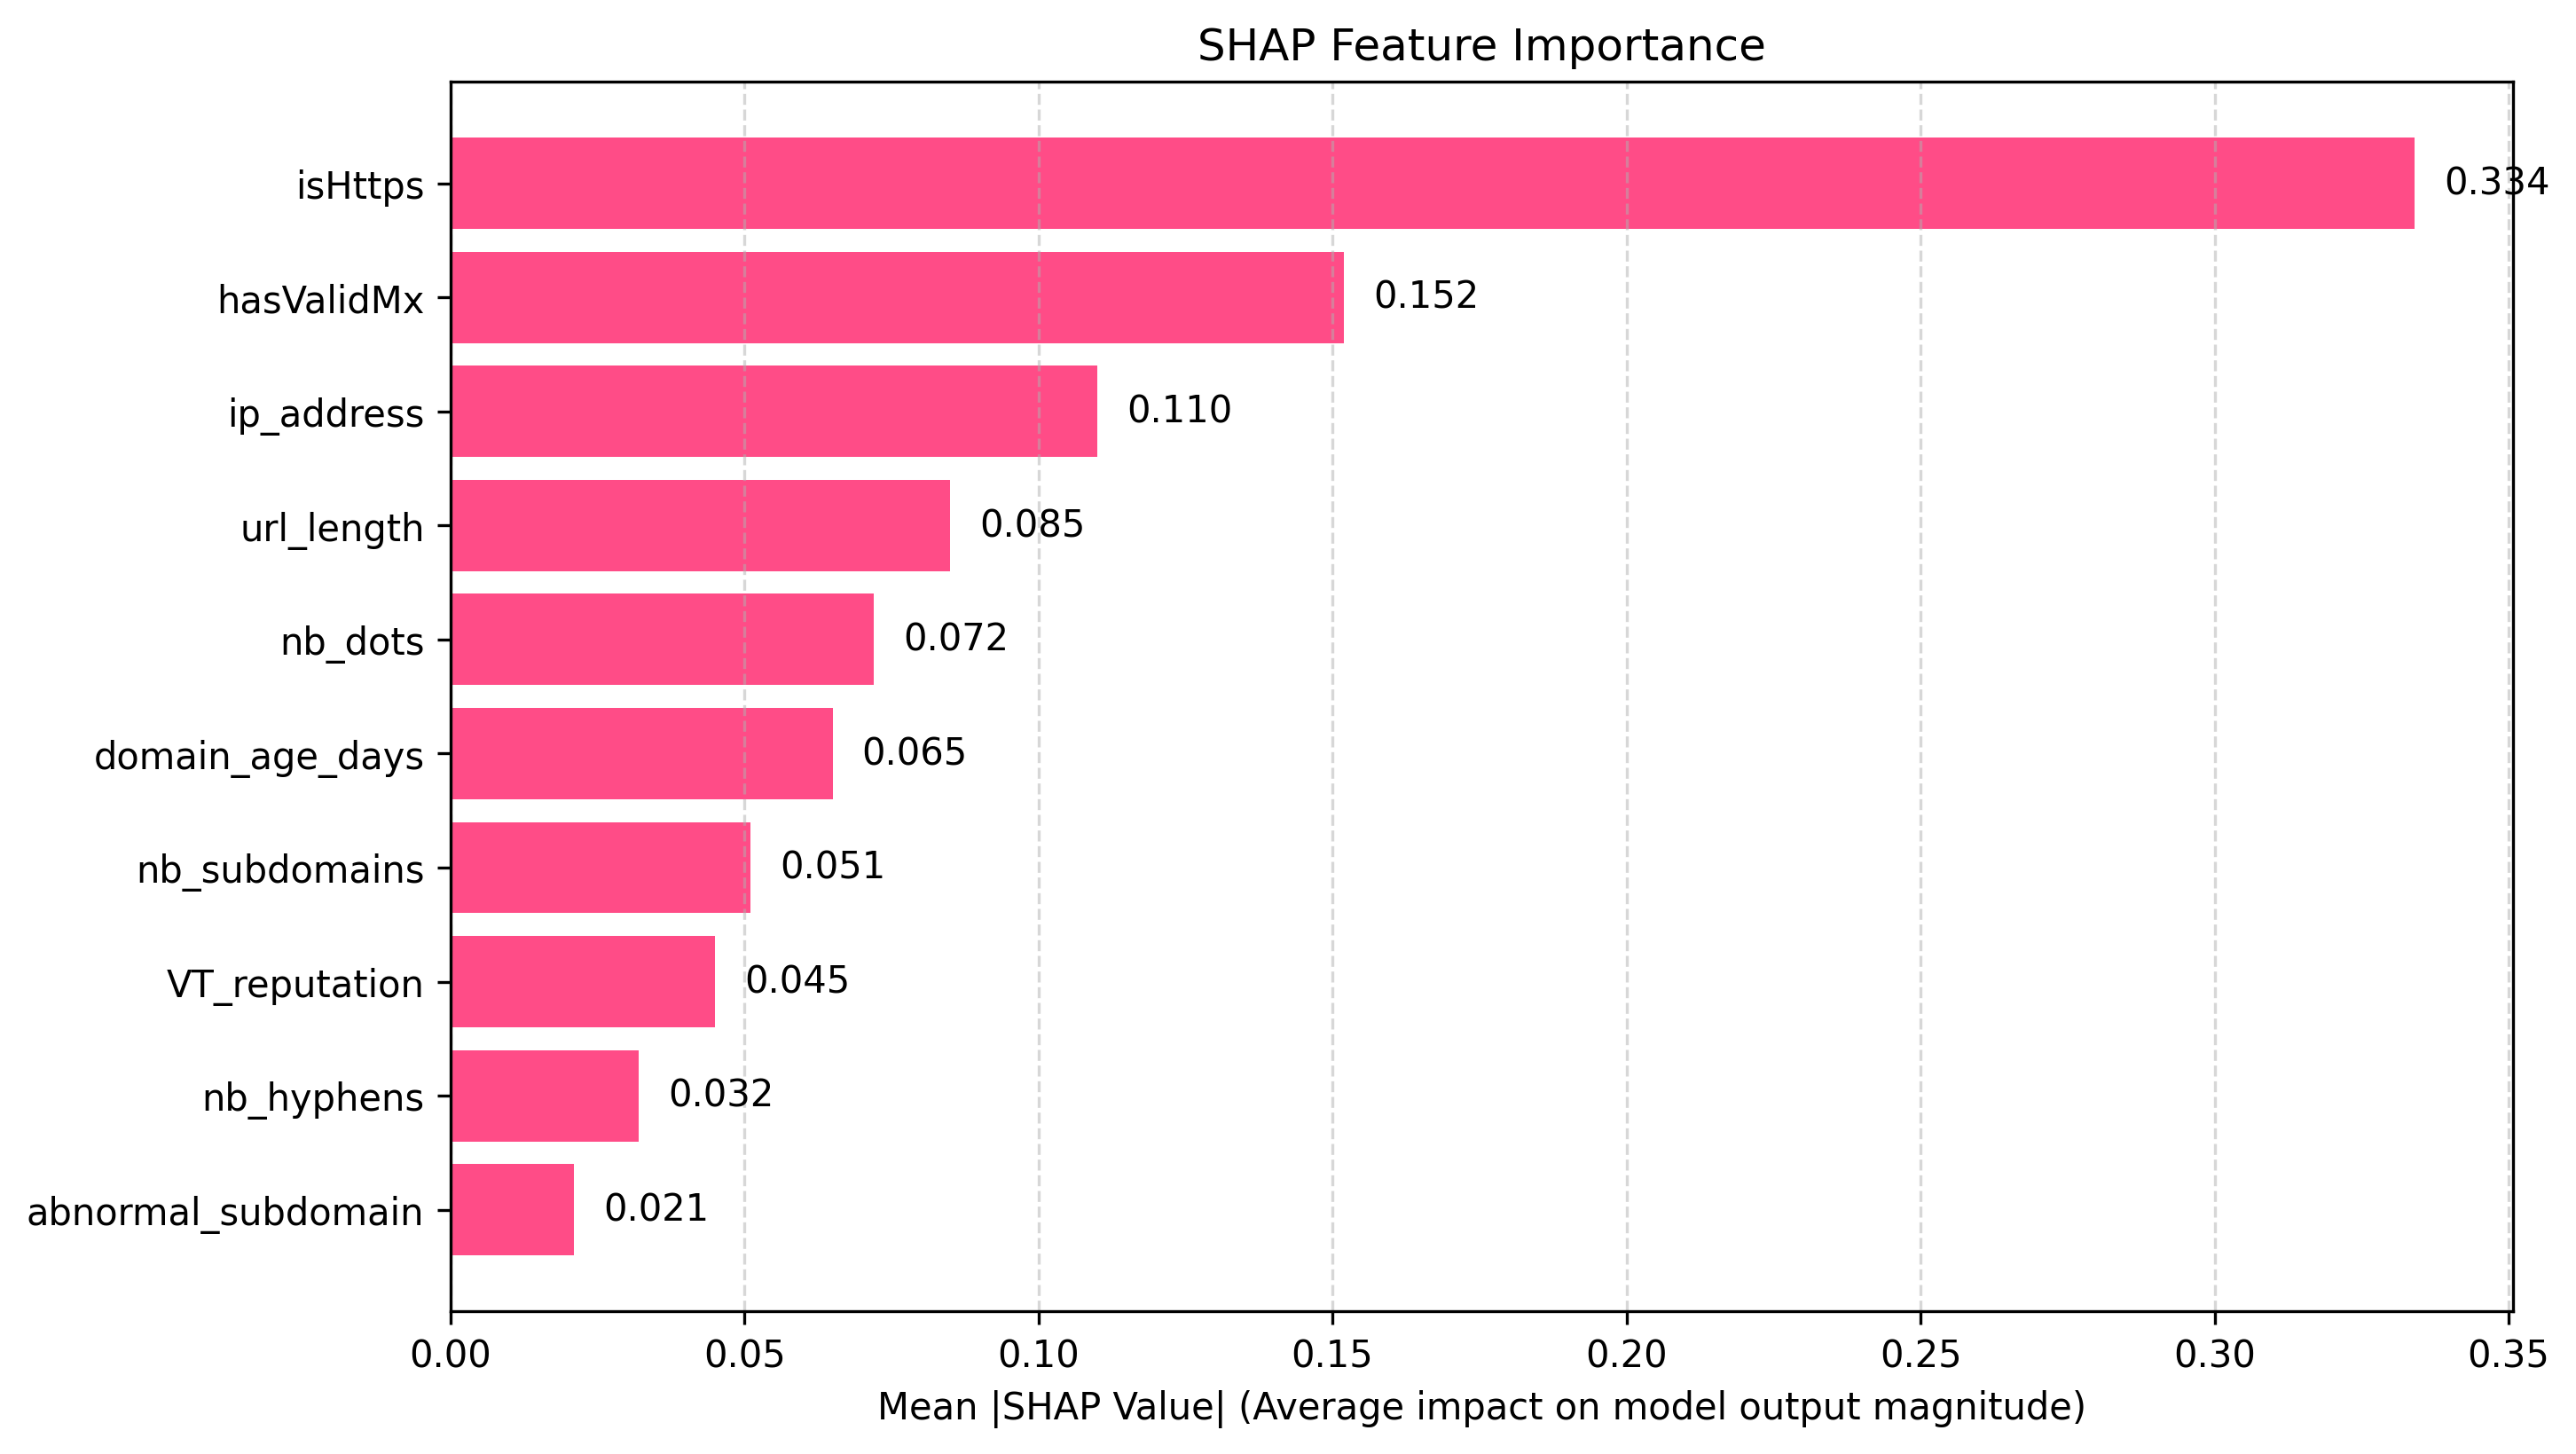
\includegraphics[height=0.32\textheight]{../latex_source/images/shap_plot.png}\\[0.4em]
        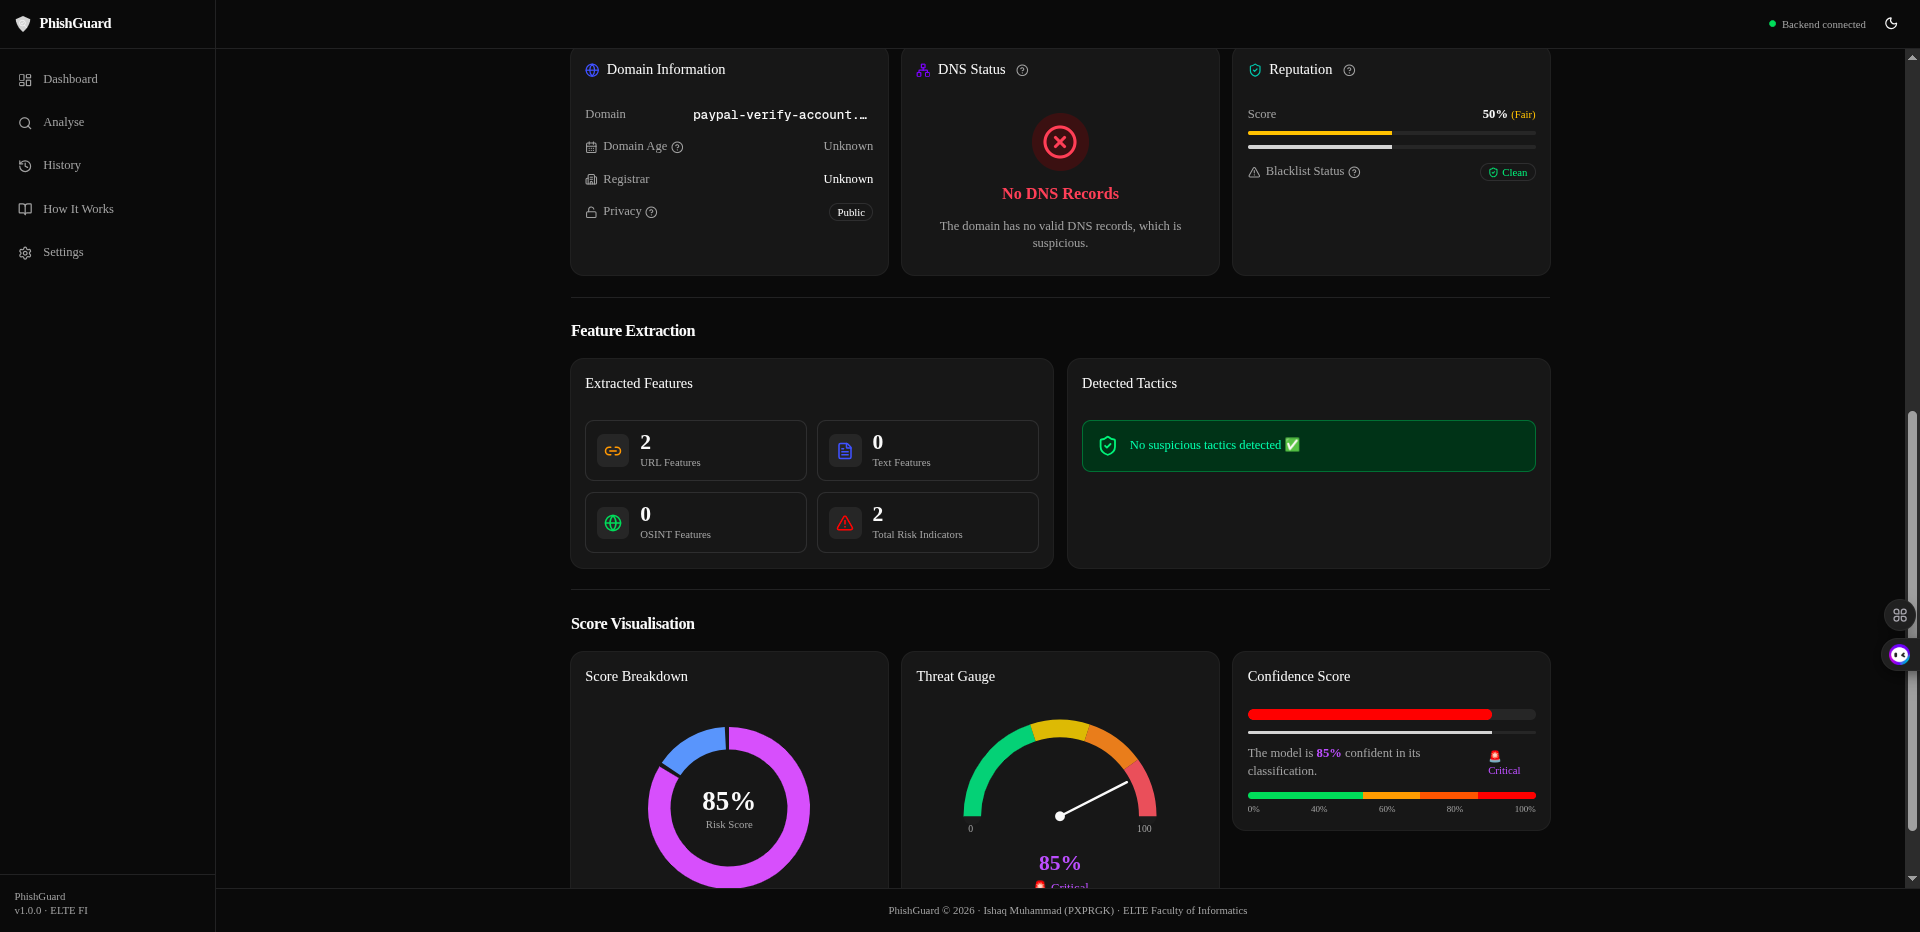
\includegraphics[height=0.32\textheight]{../latex_source/images/score-viz.png}
      \end{center}
  \end{columns}
\end{frame}

% ═══════════════════════════════════════════════════════════════════
\begin{frame}[standout]
  \Large How do we know \emph{why} it made that decision?
\end{frame}

% ═══════════════════════════════════════════════════════════════════
\begin{frame}{SHAP Explainability}
  \vspace{0.2cm}
  \begin{columns}[T]
    \column{0.48\textwidth}
      \begin{block}{What SHAP does}
        For \emph{every} prediction, SHAP calculates each feature's \textbf{marginal contribution}:
        \begin{itemize}
          \item ``\texttt{hasValidMx=False} pushed the score +0.15 toward phishing''
          \item ``\texttt{isHttps=True} pushed the score -0.08 toward safe''
        \end{itemize}
      \end{block}
      \vspace{0.3cm}
      \begin{exampleblock}{OSINT matters}
        \textbf{14.36\%} of total SHAP importance comes from the 4 OSINT features alone.
      \end{exampleblock}
    \column{0.52\textwidth}
      \begin{center}
        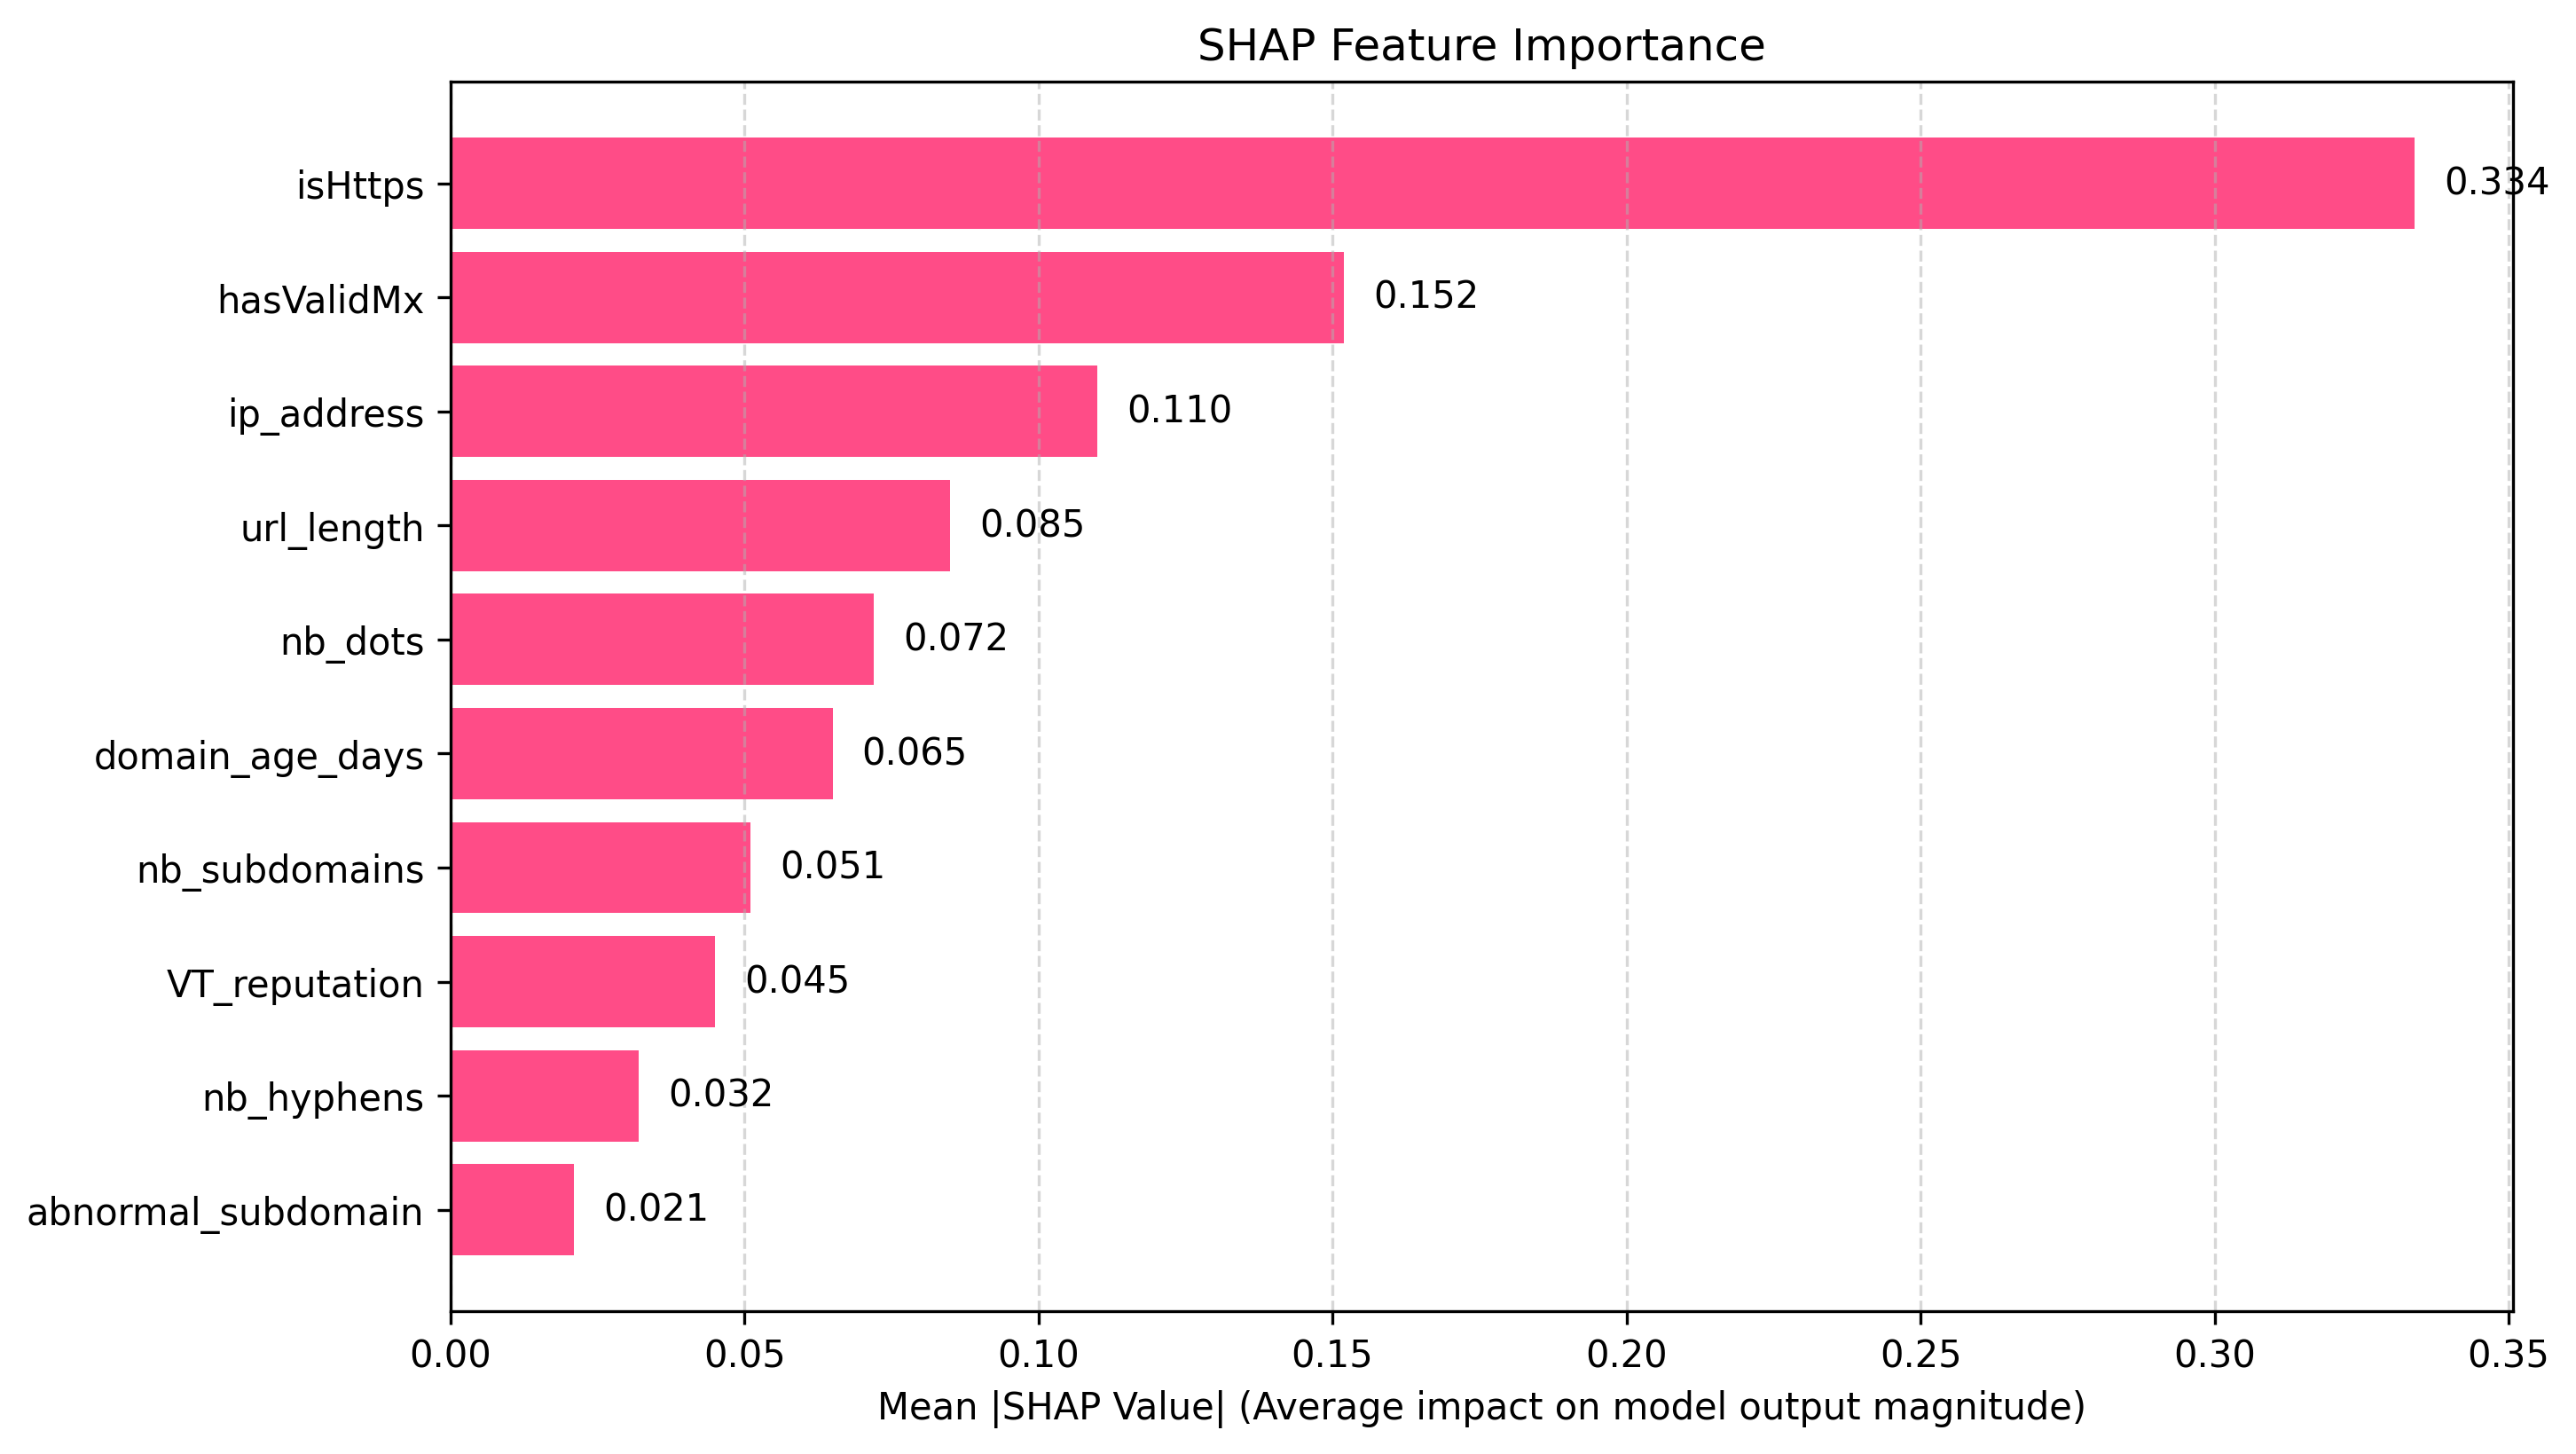
\includegraphics[height=0.65\textheight]{../latex_source/images/shap_plot.png}
      \end{center}
  \end{columns}
\end{frame}

% ═══════════════════════════════════════════════════════════════════
\begin{frame}[standout]
  \Large OSINT: Live Internet Intelligence
\end{frame}

% ═══════════════════════════════════════════════════════════════════
\begin{frame}{OSINT — Three Parallel Lookups}
  \vspace{0.2cm}
  \begin{columns}[T]
    \column{0.48\textwidth}
      \begin{block}{WHOIS}
        \begin{itemize}
          \item Domain age, registrar, expiration
          \item Privacy protection detection
          \item \textbf{Red flag:} Registered < 30 days ago
        \end{itemize}
      \end{block}
      \vspace{0.2cm}
      \begin{block}{DNS}
        \begin{itemize}
          \item A, AAAA, MX, NS, TXT, CNAME
          \item CDN detection (Cloudflare, Akamai, \ldots)
          \item \textbf{Red flag:} No MX records configured
        \end{itemize}
      \end{block}
      \vspace{0.2cm}
      \begin{block}{Reputation}
        \begin{itemize}
          \item VirusTotal (70+ engines)
          \item AbuseIPDB
          \item \textbf{Red flag:} Flagged by multiple sources
        \end{itemize}
      \end{block}
    \column{0.52\textwidth}
      \begin{center}
        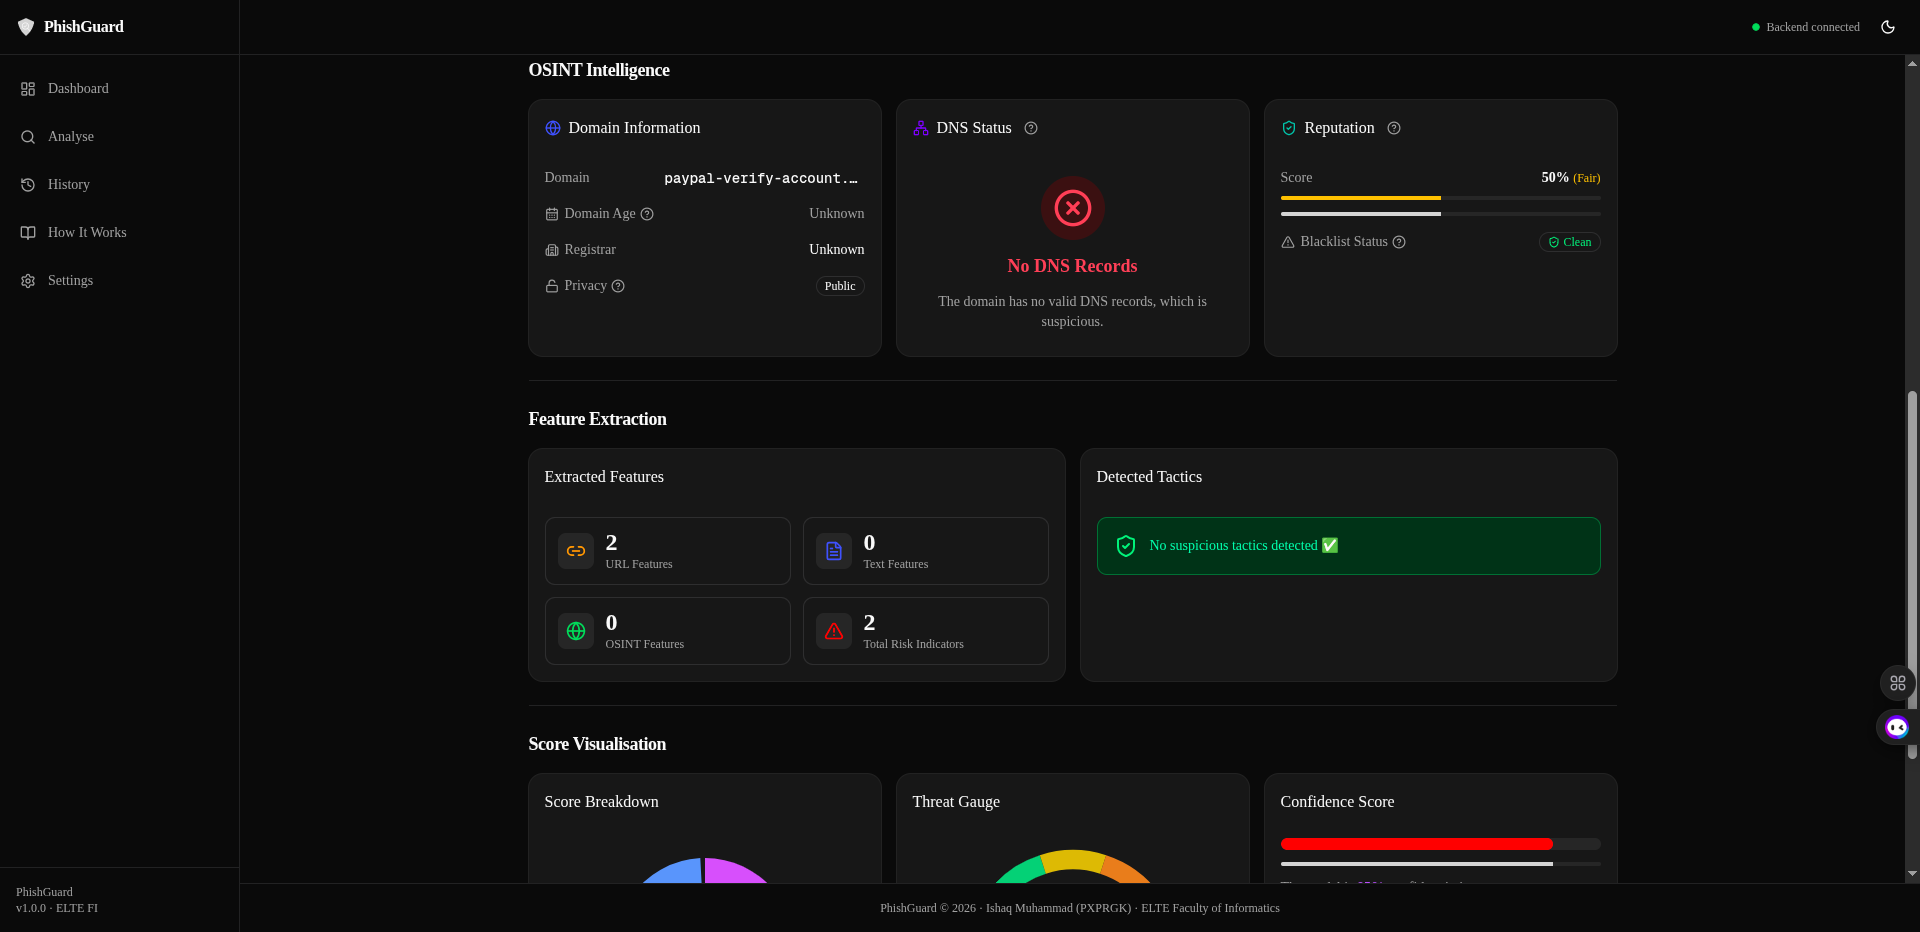
\includegraphics[height=0.7\textheight]{../latex_source/images/osint-results.png}
      \end{center}
  \end{columns}
  \vspace{0.2cm}
  \begin{center}
    \small\textbf{15-second global timeout · \texttt{asyncio.gather} parallel execution · Graceful degradation}
  \end{center}
\end{frame}

% ═══════════════════════════════════════════════════════════════════
\begin{frame}[standout]
  \Large NLP: Detecting Social Engineering
\end{frame}

% ═══════════════════════════════════════════════════════════════════
\begin{frame}{NLP — 10 Tactic Detectors}
  \vspace{0.3cm}
  \begin{columns}[T]
    \column{0.52\textwidth}
      \begin{block}{spaCy PhraseMatcher — Rule-Based}
        \begin{enumerate}
          \setlength{\itemsep}{0.3em}
          \item \textbf{Urgency} — \textit{``act now'', ``24 hours''}
          \item \textbf{Threats} — \textit{``account suspended''}
          \item \textbf{Authority} — \textit{``IT department''}
          \item \textbf{Brands} — \textit{PayPal, Microsoft, IRS}
          \item \textbf{Credentials} — \textit{``verify password''}
          \item \textbf{Actions} — \textit{``click here''}
          \item \textbf{Emotion} — \textit{``congratulations!''}
          \item \textbf{Money} — \textit{``wire transfer''}
          \item \textbf{Social Proof} — \textit{``millions of users''}
          \item \textbf{Attachments} — regex patterns
        \end{enumerate}
      \end{block}
    \column{0.48\textwidth}
      \vspace{0.3cm}
      \begin{exampleblock}{Why rule-based?}
        \begin{itemize}
          \setlength{\itemsep}{0.3em}
          \item \textbf{Deterministic} — same input, same output
          \item \textbf{Explainable} — exact text evidence
          \item \textbf{Fast} — CPU, milliseconds
          \item \textbf{Maintainable} — add phrases, no retrain
        \end{itemize}
      \end{exampleblock}
      \vspace{0.5cm}
      \begin{block}{Scoring Weights}
        \begin{tabular}{@{}lll@{}}
          \toprule
          Mode & Primary & Secondary \\
          \midrule
          URL & ML: \textbf{85\%} & NLP: 15\% \\
          Email & NLP: \textbf{55\%} & URL 25\% + OSINT 20\% \\
          \bottomrule
        \end{tabular}
      \end{block}
  \end{columns}
\end{frame}

% ═══════════════════════════════════════════════════════════════════
\begin{frame}[standout]
  \Large The Application
\end{frame}

% ═══════════════════════════════════════════════════════════════════
\begin{frame}{Live Demo Screens}
  \vspace{-0.2cm}
  \begin{columns}[T]
    \column{0.48\textwidth}
      \begin{center}
        \fbox{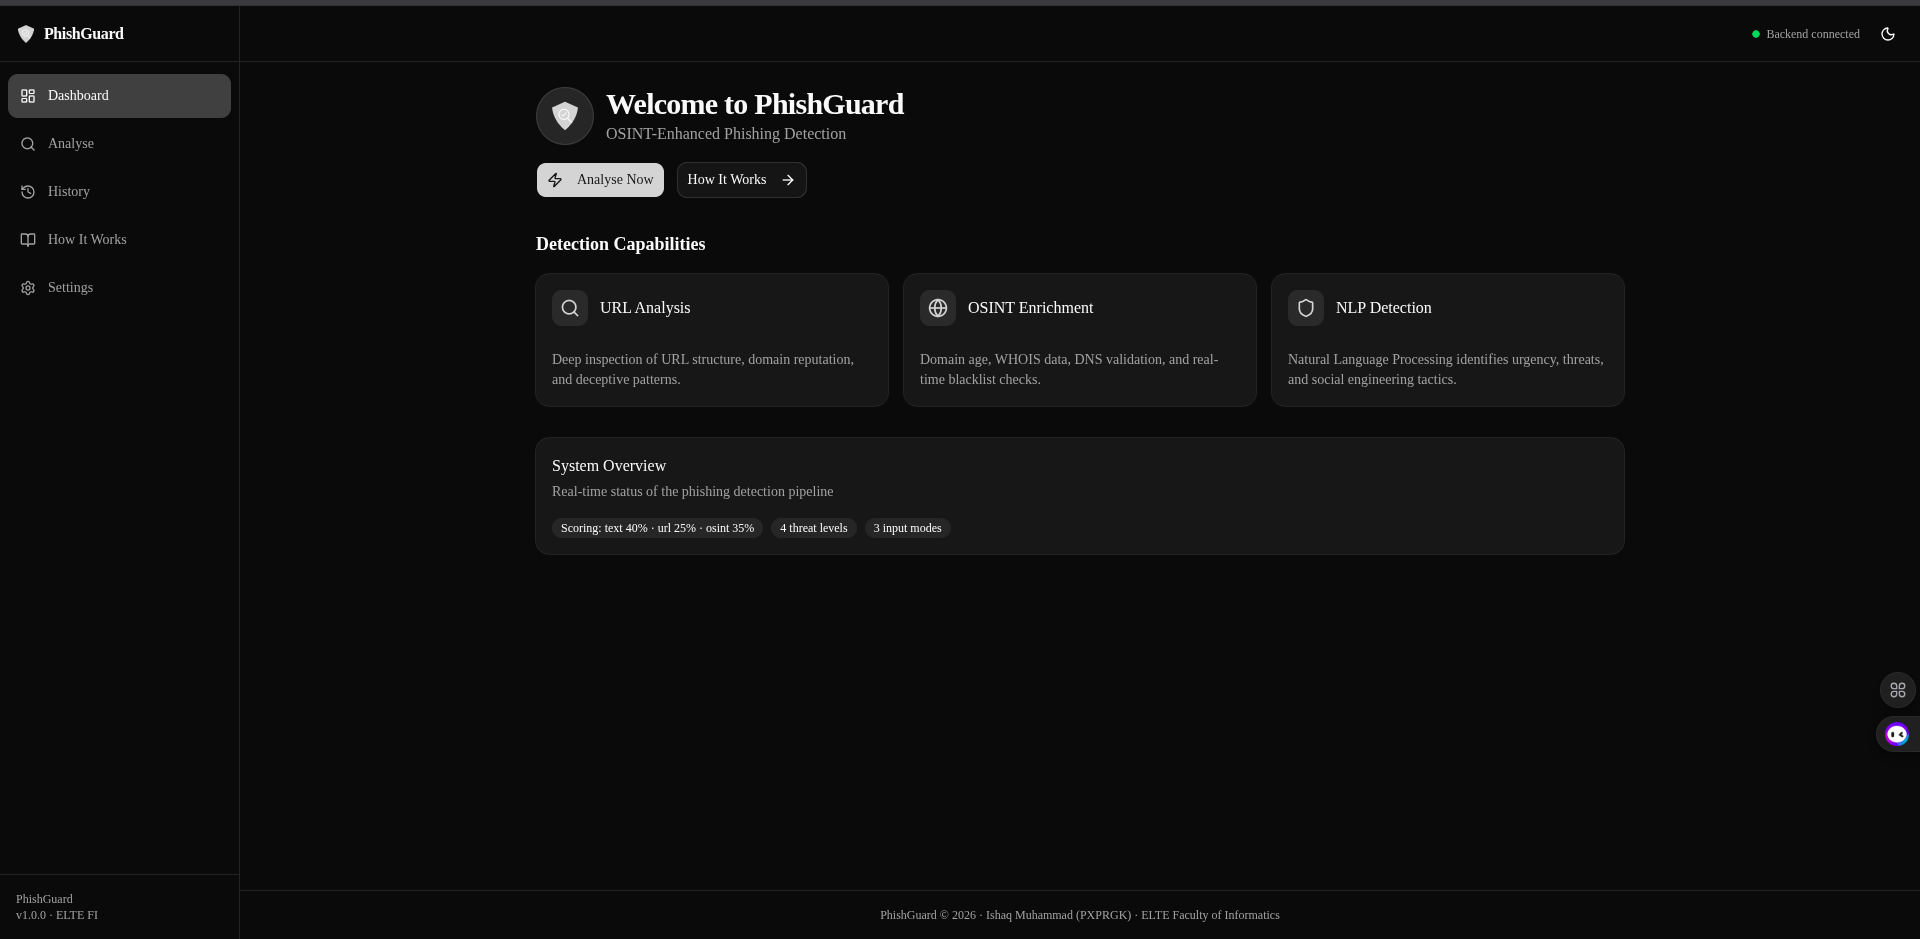
\includegraphics[width=\textwidth]{../latex_source/images/dashboard.png}}\\[0.2em]
        {\small Dashboard}
      \end{center}
    \column{0.48\textwidth}
      \begin{center}
        \fbox{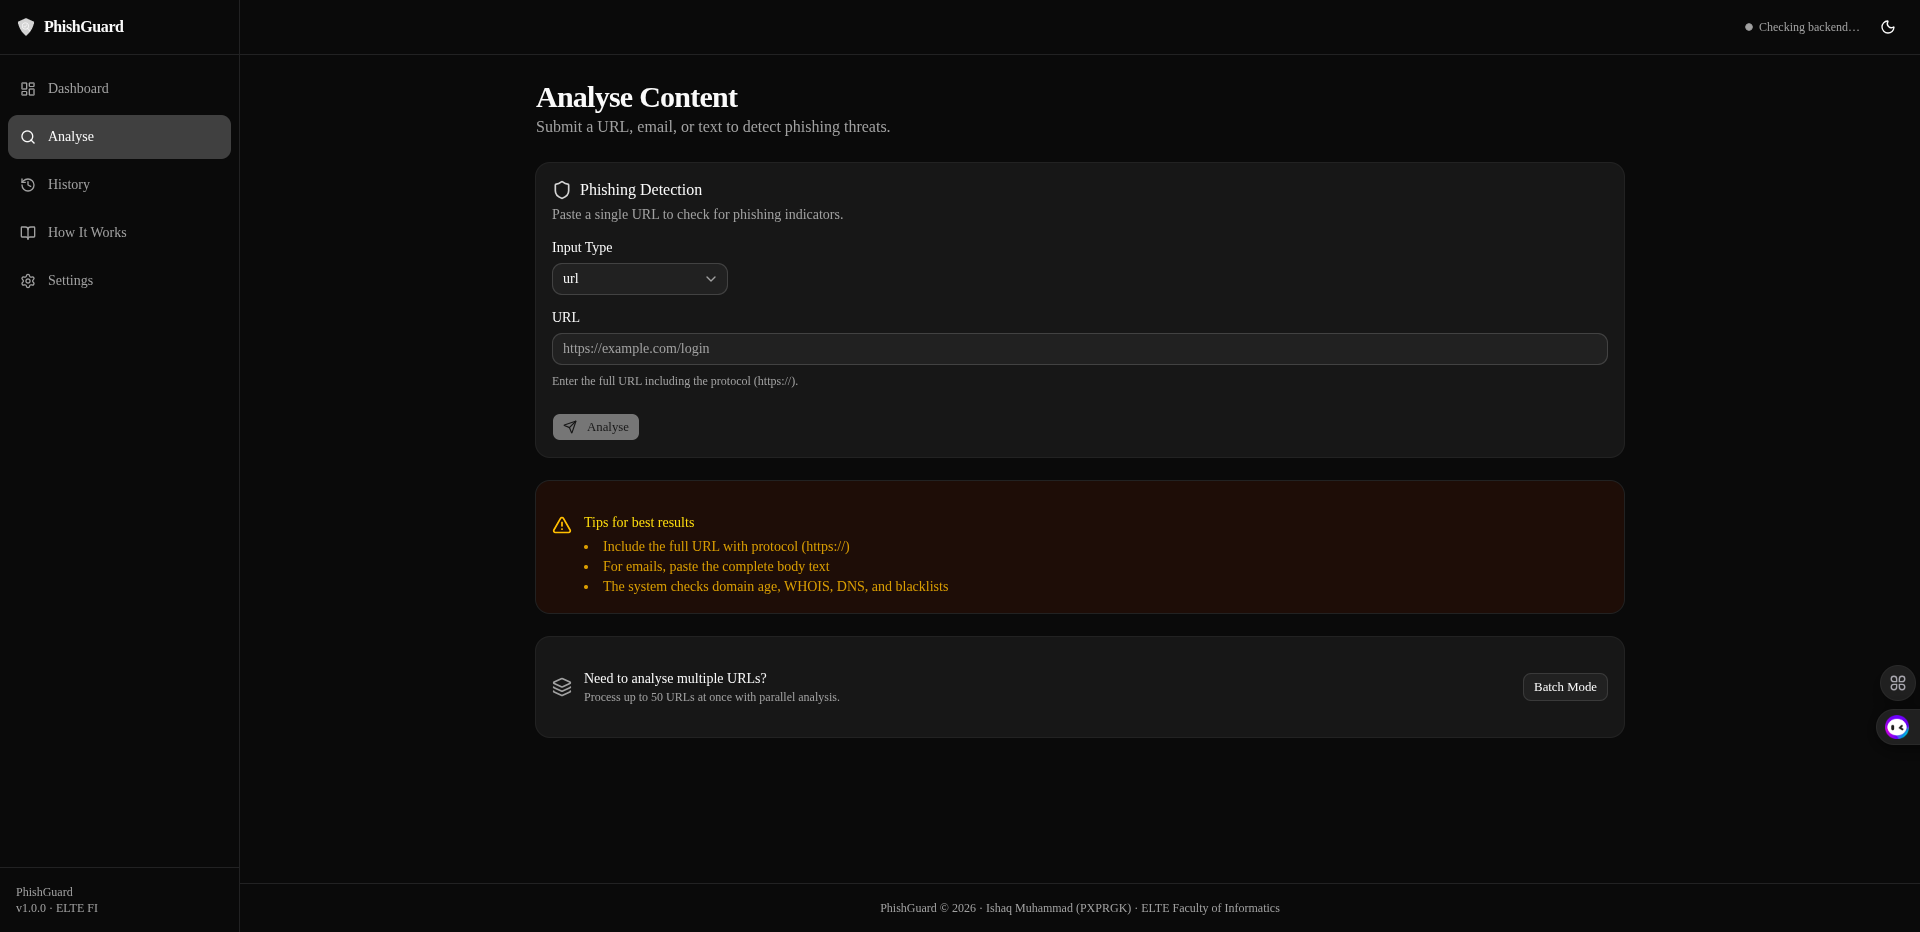
\includegraphics[width=\textwidth]{../latex_source/images/analyze-page.png}}\\[0.2em]
        {\small Analyze — URL / Email / Text}
      \end{center}
  \end{columns}
  \vspace{0.3cm}
  \begin{columns}[T]
    \column{0.48\textwidth}
      \begin{center}
        \fbox{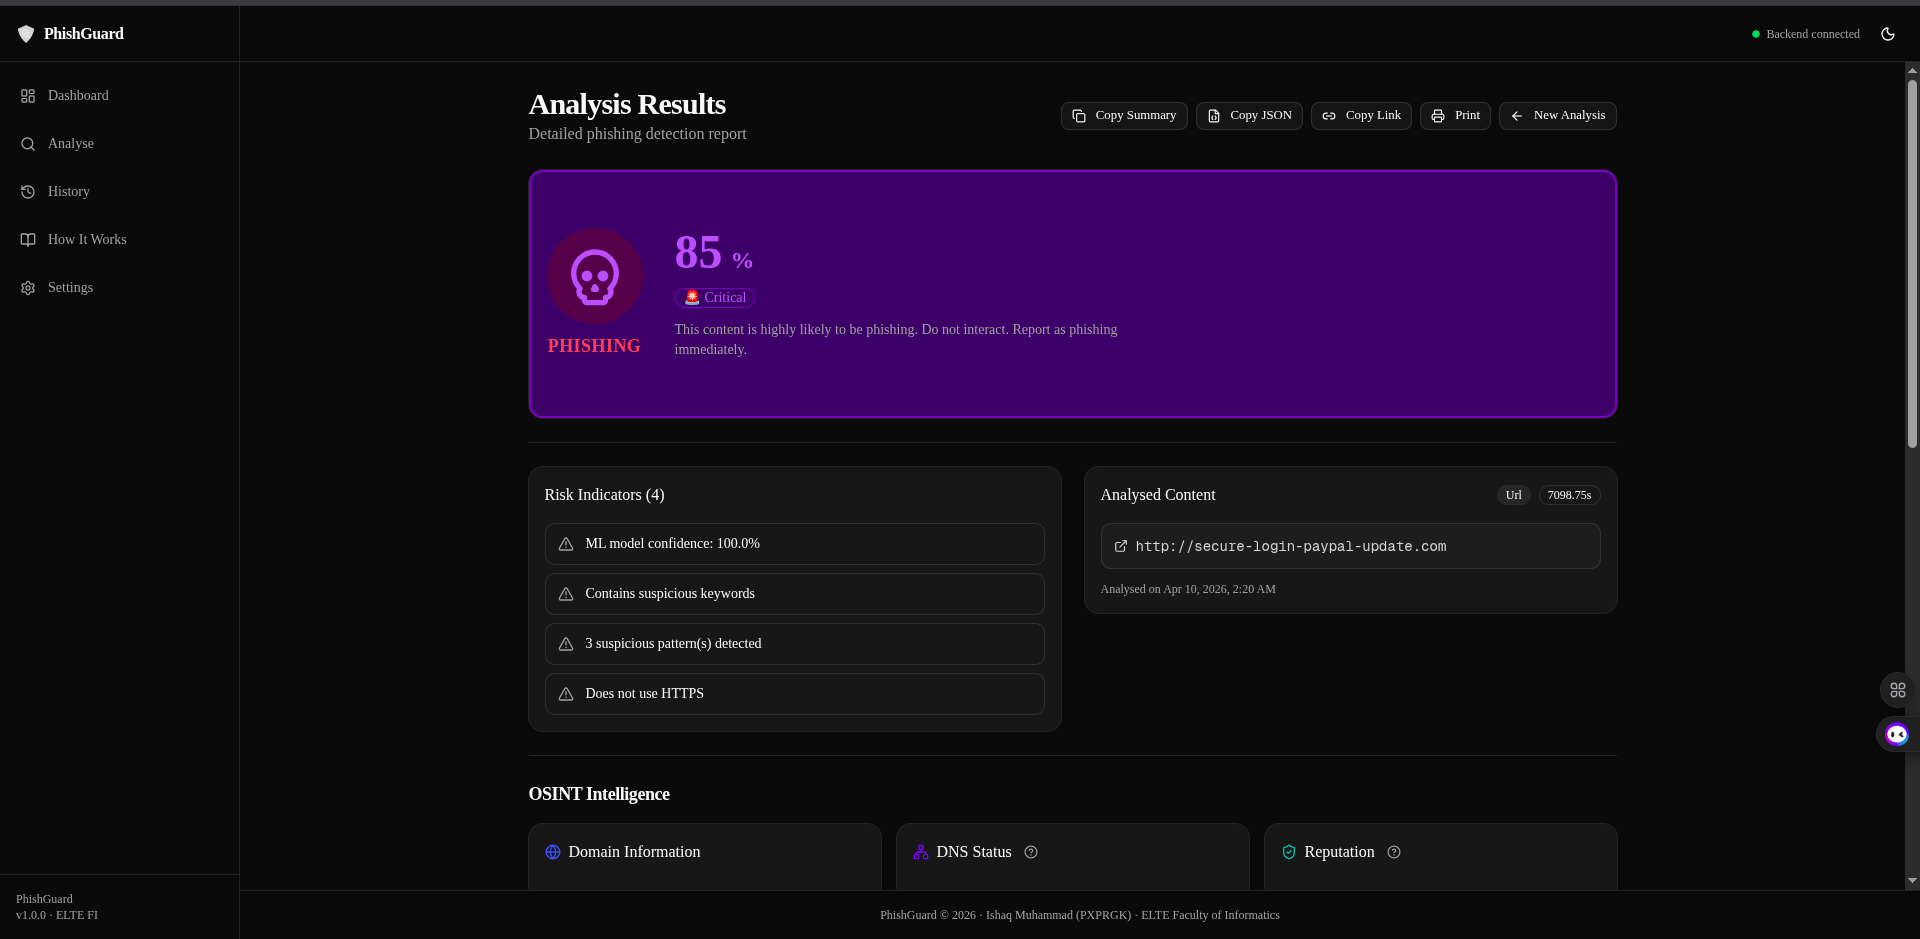
\includegraphics[width=\textwidth]{../latex_source/images/result.png}}\\[0.2em]
        {\small Results — Verdict, OSINT, Reasons}
      \end{center}
    \column{0.48\textwidth}
      \begin{center}
        \fbox{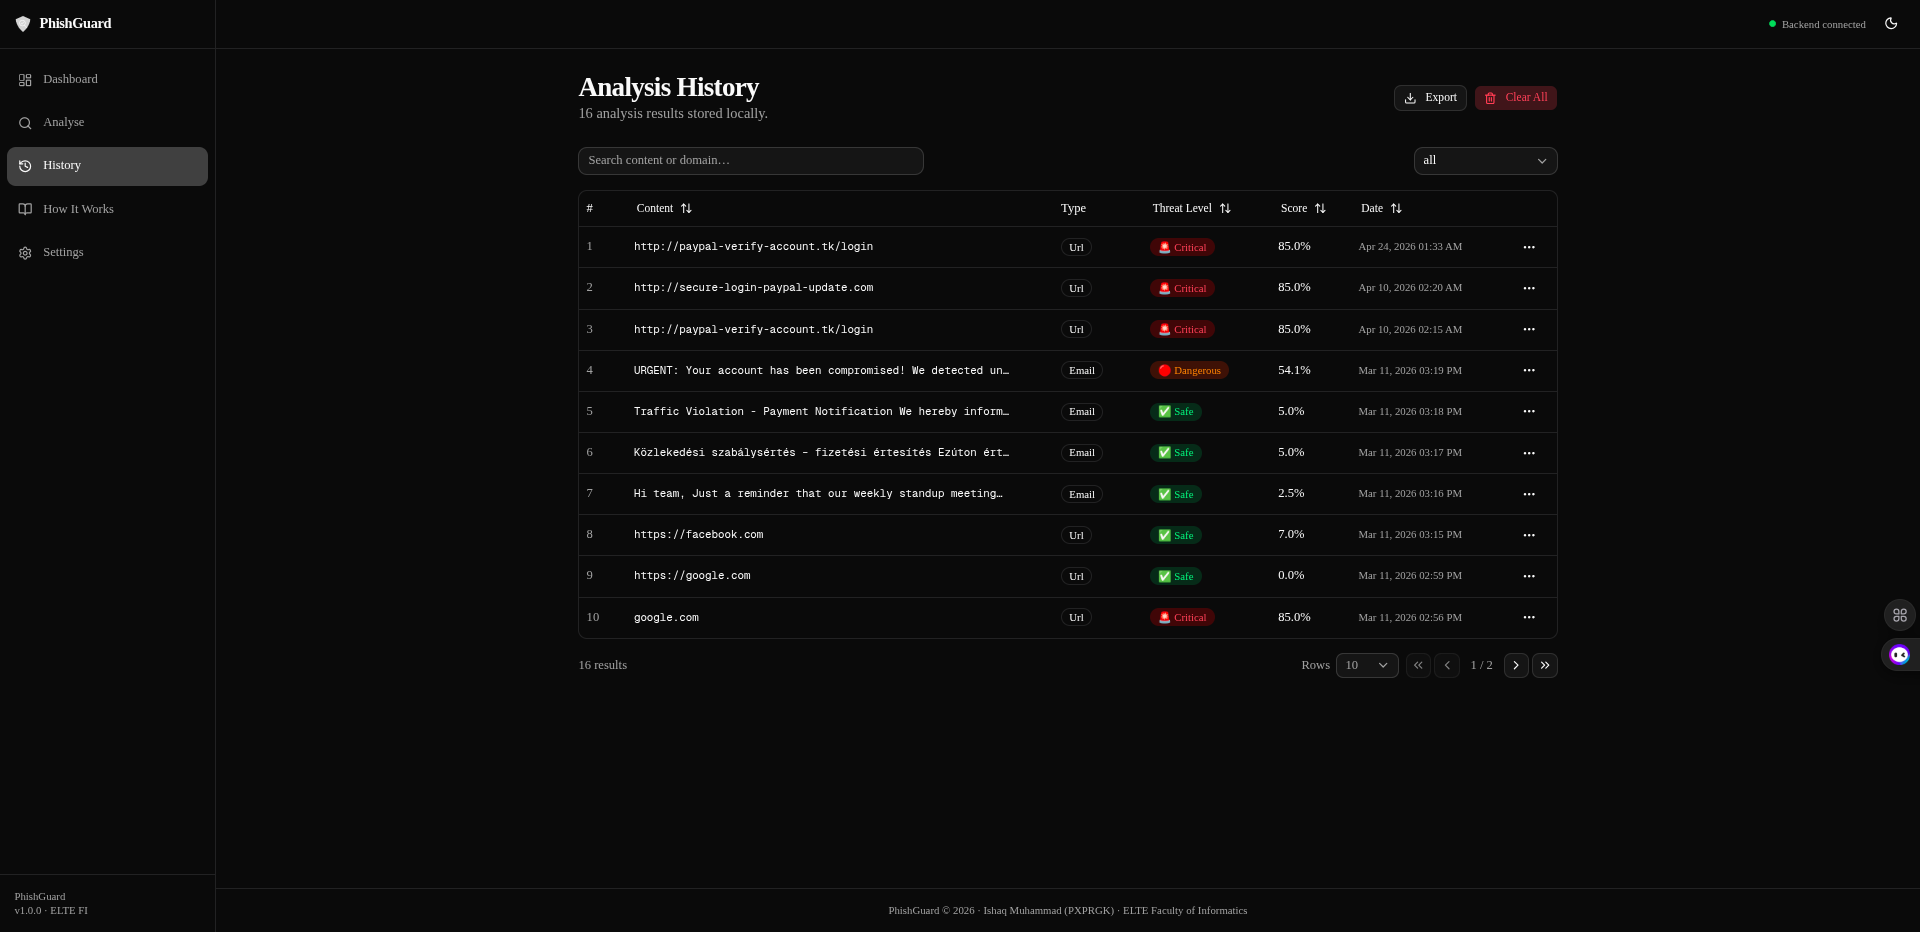
\includegraphics[width=\textwidth]{../latex_source/images/history-page.png}}\\[0.2em]
        {\small History — localStorage, no account needed}
      \end{center}
  \end{columns}
\end{frame}

% ═══════════════════════════════════════════════════════════════════
\begin{frame}{Full Tech Stack \& Deployment}
  \vspace{0.3cm}
  \begin{columns}[T]
    \column{0.45\textwidth}
      \begin{block}{Backend}
        \begin{itemize}
          \item \textbf{FastAPI} — async Python REST API
          \item \textbf{XGBoost} — gradient boosting classifier
          \item \textbf{spaCy 3.7} — NLP engine
          \item \textbf{WHOIS + DNS + Reputation} — OSINT
          \item Deployed on \textbf{Render}
        \end{itemize}
      \end{block}
      \vspace{0.3cm}
      \begin{block}{Testing}
        \begin{itemize}
          \item \textbf{592} pytest (backend)
          \item \textbf{133} Jest (frontend)
          \item \textbf{28} Playwright E2E
          \item Total: \textbf{725+} automated tests
        \end{itemize}
      \end{block}
    \column{0.45\textwidth}
      \begin{block}{Frontend}
        \begin{itemize}
          \item \textbf{Next.js 16} — React framework
          \item \textbf{Tailwind CSS v4 + shadcn/ui}
          \item \textbf{Recharts} — data visualization
          \item \textbf{TanStack Table} — history table
          \item Deployed on \textbf{Vercel}
        \end{itemize}
      \end{block}
      \vspace{0.3cm}
      \begin{exampleblock}{Live URLs}
        \small
        \texttt{project-4soy4.vercel.app}\\
        \texttt{phishguard-api-upl2.onrender.com}\\
        \texttt{github.com/ishaq2321/phishing-detection-osint}
      \end{exampleblock}
  \end{columns}
\end{frame}

% ═══════════════════════════════════════════════════════════════════
\begin{frame}{Contributions}
  \vspace{0.2cm}
  \begin{enumerate}
    \setlength{\itemsep}{0.6em}
    \item \textbf{OSINT-Enhanced Feature Engineering}\\
      {\small 4 live infrastructure features fused into the ML vector — 14.36\% SHAP contribution}
    \item \textbf{High-Performance XGBoost Pipeline}\\
      {\small 96.45\% accuracy, 99.41\% AUC — Optuna-optimized with 50 trials}
    \item \textbf{SHAP Explainability Layer}\\
      {\small Every prediction comes with per-feature contribution scores and human-readable reasons}
    \item \textbf{Multi-Modal Analysis Engine}\\
      {\small Auto-detects URL / email / text — routes through ML or NLP pipeline dynamically}
    \item \textbf{Production Full-Stack Application}\\
      {\small Next.js + FastAPI, 725 tests, live cloud deployment, Swagger docs}
  \end{enumerate}
\end{frame}

% ═══════════════════════════════════════════════════════════════════
\begin{frame}{Future Work}
  \vspace{0.3cm}
  \begin{columns}[T]
    \column{0.48\textwidth}
      \begin{block}{Algorithmic}
        \begin{itemize}
          \setlength{\itemsep}{0.4em}
          \item Online learning for \textbf{concept drift}
          \item Integration of \textbf{LLMs} for deeper semantic analysis
          \item \textbf{OCR} for image-based phishing
        \end{itemize}
      \end{block}
    \column{0.48\textwidth}
      \begin{block}{Engineering}
        \begin{itemize}
          \setlength{\itemsep}{0.4em}
          \item \textbf{Browser extension} for real-time protection
          \item \textbf{CI/CD pipeline} with automated test gates
          \item \textbf{Database} persistence (PostgreSQL)
          \item \textbf{Docker} containerization
        \end{itemize}
      \end{block}
  \end{columns}
\end{frame}

% ═══════════════════════════════════════════════════════════════════
\begin{frame}[standout]
  \Huge Thank You\\[0.3em]
  \Large Questions \& Discussion\\[0.8em]
  \normalsize
  Ishaq Muhammad · PXPRGK\\[0.2em]
  pxprgk@inf.elte.hu\\[0.4em]
  {\footnotesize github.com/ishaq2321/phishing-detection-osint}
\end{frame}

\end{document}
